\documentclass[12pt,a4paper]{article}
\usepackage[T1]{fontenc}
\usepackage[utf8]{inputenc}
\usepackage[margin=1in]{geometry}
\usepackage{graphicx}
\usepackage{array}
\usepackage{tabularx}
\usepackage{booktabs}
\usepackage{hyperref}
\usepackage{float}
\usepackage{amsmath}
\usepackage{xcolor}
\usepackage{listings}
\usepackage{fancyhdr}
\usepackage{ragged2e}
\usepackage{tikz}
\usetikzlibrary{arrows.meta,positioning,shapes.geometric}

\hypersetup{colorlinks=true, linkcolor=black, urlcolor=blue}
% Images resolve from the report folder first, then from ./figures/
\graphicspath{{./}{figures/}}
\setlength{\parindent}{0pt}
\setlength{\parskip}{5pt}

% ---------- Header / Footer ----------
\pagestyle{fancy}
\fancyhf{}
\fancyhead[L]{\small Konkan Vani -- NLP Mini Project}
\fancyhead[R]{\small Dept. of Computer Engineering, SFIT}
\fancyfoot[C]{\small Page \thepage}
\renewcommand{\headrulewidth}{0.4pt}

% ---------- Code listing style ----------
\lstset{
  language=Python,
  basicstyle=\ttfamily\footnotesize,
  keywordstyle=\color{blue!70!black},
  commentstyle=\color{green!40!black},
  stringstyle=\color{red!60!black},
  frame=single,
  breaklines=true,
  columns=fullflexible,
  showstringspaces=false
}

% ---------- Safe figure: shows a placeholder box if the image file is missing ----------
\newcommand{\safefig}[2]{%
  \IfFileExists{#1}{\includegraphics[#2]{#1}}{%
    \fbox{\parbox[c][5cm][c]{0.85\linewidth}{\centering\small Screenshot placeholder:\\ \texttt{\detokenize{#1}}}}}%
}

% ---------- TikZ styles for flowcharts ----------
\tikzset{
  proc/.style={draw, rounded corners, minimum width=4.2cm, minimum height=0.9cm, align=center, font=\small},
  dec/.style={draw, diamond, aspect=2.4, align=center, font=\scriptsize, inner sep=1pt},
  io/.style={draw, trapezium, trapezium left angle=70, trapezium right angle=110, minimum height=0.9cm, align=center, font=\small},
  arr/.style={-{Latex}, thick}
}

\let\oldsection\section
\renewcommand{\section}{\clearpage\oldsection}

\begin{document}

% =====================================================
% a) TITLE PAGE
% =====================================================
\begin{titlepage}
\thispagestyle{empty}
\centering

{\Large\bfseries St. Francis Institute of Technology}\\[2pt]
(Engineering College)\\[2pt]
{\small\bfseries An Autonomous Institute, Affiliated to University of Mumbai}\\[2pt]
{\scriptsize NAAC A+ Accredited $|$ CMPN, EXTC, INFT NBA Accredited $|$ ISO 9001:2015 Certified}\\[6pt]
{\large\bfseries Department of Computer Engineering}\\
\vspace{0.5cm}
\includegraphics[width=3.5cm]{logo.png}

\vspace{1.2cm}

{\LARGE\bfseries Mini Project Report}\\[6pt]
{\large Subject: Natural Language Processing}\\[10pt]

\vspace{1.5cm}
{\Large\bfseries Konkan Vani}\\[6pt]
{\large\bfseries A Bilingual Konkani Idiom and\\Proverb Meaning Retrieval System}

\vspace{1.8cm}
{\large\bfseries Group Members}\\[8pt]
\renewcommand{\arraystretch}{1.5}
\begin{tabular}{|c|p{7cm}|c|}
\hline
\textbf{Sr. No.} & \textbf{Name of Student} & \textbf{Roll No.} \\
\hline
1 & Siddhant Sawant & 26 \\
\hline
2 & Krishna Sharma & 31 \\
\hline
3 & Kshitij Sharma & 32 \\
\hline
\end{tabular}

\vspace{1.5cm}
{\large Under the guidance of}\\[4pt]
{\large\bfseries Prof. Pradnya Sawant}

\vfill
{\large Academic Year: 2026--2027}
\end{titlepage}

\pagenumbering{roman}

% =====================================================
% CERTIFICATE
% =====================================================
\section*{\centering Certificate}
\addcontentsline{toc}{section}{Certificate}

\vspace{0.5cm}
\begin{center}
\textbf{Department of Computer Engineering}\\
St. Francis Institute of Technology, Mumbai
\end{center}
\vspace{0.5cm}

\begin{justify}
This is to certify that the NLP mini project report entitled ``\textbf{Konkan Vani: A Bilingual Konkani Idiom and Proverb Meaning Retrieval System}'' has been satisfactorily completed by \textbf{Siddhant Sawant (Roll No.\ 26)}, \textbf{Krishna Sharma (Roll No.\ 31)}, and \textbf{Kshitij Sharma (Roll No.\ 32)} of the Department of Computer Engineering, St. Francis Institute of Technology, Mumbai, during the academic year 2026--2027, in partial fulfilment of the requirements for the degree of Bachelor of Engineering in Computer Engineering of the University of Mumbai.
\end{justify}

\vspace{3cm}
\noindent
\begin{tabularx}{\textwidth}{XX}
\textbf{Project Guide} & \textbf{Head of Department}\\[0.3cm]
Prof. Pradnya Sawant & [Name of HOD]\\[2.5cm]
\textbf{Date:} & \textbf{Place:} Mumbai\\
\end{tabularx}
\newpage

% =====================================================
% DECLARATION
% =====================================================
\section*{\centering Declaration}
\addcontentsline{toc}{section}{Declaration}

\vspace{0.5cm}
\begin{justify}
We declare that this written submission, entitled ``Konkan Vani: A Bilingual Konkani Idiom and Proverb Meaning Retrieval System'', represents our own ideas and work in our own words. Wherever the ideas, data, or words of others have been included, we have cited and referenced the original sources. We also declare that we have adhered to all principles of academic honesty and integrity and have not misrepresented, fabricated, or falsified any idea, data, fact, or source in this submission. We understand that any violation of the above will be cause for disciplinary action by the Institute.
\end{justify}

\vspace{2cm}
\noindent\textbf{Student signatures:}\\[1.5cm]
\begin{tabularx}{\textwidth}{XXX}
\rule{4.2cm}{0.4pt} & \rule{4.2cm}{0.4pt} & \rule{4.2cm}{0.4pt}\\
Siddhant Sawant (26) & Krishna Sharma (31) & Kshitij Sharma (32)\\
\end{tabularx}

\vspace{1.5cm}
\noindent\textbf{Date:}\hspace{6cm}\textbf{Place:} Mumbai
\newpage

% =====================================================
% ACKNOWLEDGEMENT
% =====================================================
\section*{\centering Acknowledgement}
\addcontentsline{toc}{section}{Acknowledgement}

\vspace{0.5cm}
\begin{justify}
We express our sincere gratitude to our project guide, Prof. Pradnya Sawant, for her valuable guidance, encouragement, and constructive feedback throughout the development of this mini project. We thank the Head of the Department and the faculty of the Department of Computer Engineering, St. Francis Institute of Technology, for providing the opportunity and resources to study natural language processing through a practical application.

We also acknowledge the authors and maintainers of the open-source tools and models used in this work, including Next.js, FastAPI, SentenceTransformers (LaBSE), FAISS, and RapidFuzz, as well as the communities behind the public Konkani language resources that informed this project's vocabulary and idiom collection.

Finally, we thank our families and friends for their constant support during the course of this work.
\end{justify}

\vspace{1.5cm}
\hfill
\begin{tabular}{l}
Siddhant Sawant\\
Krishna Sharma\\
Kshitij Sharma
\end{tabular}
\newpage
% =====================================================
% ABSTRACT  (updated with real fine-tuning + measured results)
% =====================================================
\section*{\centering Abstract}
\addcontentsline{toc}{section}{Abstract}

\vspace{0.5cm}
\begin{justify}
Konkan Vani is a web-based natural language processing (NLP) system that helps users retrieve the meanings of Konkani idioms and proverbs. Konkani is written in several scripts and is often typed informally, so the same idiom appears in many spellings, and users frequently remember only what an idiom means rather than how it is written. The system accepts queries in Devanagari, Kannada-script, Romanized Konkani, and English or Marathi descriptions of a meaning.

A Next.js web client communicates with a Python FastAPI service that resolves each query through a staged pipeline: phonetic normalization with RapidFuzz fuzzy matching, multilingual semantic retrieval using a LaBSE-based encoder fine-tuned on Konkani idiom data (konkan-vani-encoder-v1), and a FAISS vector index, followed by a compositional fallback that glosses the query word by word and composes a provisional meaning when no stored idiom qualifies. For each retrieved idiom the interface presents the literal meaning, figurative meaning, English and Marathi meanings, and an example sentence.

The system is built on a dataset of 5,200 idiom records, each encoded as a 768-dimensional embedding. Fine-tuning the encoder with MultipleNegativesRankingLoss on 8,320 in-domain pairs raised held-out retrieval performance from a LaBSE Recall@1 of 51.4\% to 99.8\% (MRR@10 from 62.8\% to 99.8\%). In an automated benchmark on the live system, 200 sampled in-domain queries were retrieved with 100\% top-1 accuracy despite corrupted spellings, 150 Romanized and 150 Devanagari full-pipeline queries were each resolved correctly in 100\% of cases, and eight unrelated out-of-domain queries were all rejected with no false positives. Fuzzy matching takes about 3\,ms and full query resolution about 35\,ms (95th percentile 47\,ms) on a CUDA machine. The project shows that combining lexical and semantic retrieval with a domain fine-tuned encoder is an effective way to make Konkani idiomatic knowledge searchable across scripts and spelling conventions.
\end{justify}

\vspace{0.5cm}
\noindent\textbf{Keywords:} Natural Language Processing, Konkani, idiom retrieval, multilingual embeddings, LaBSE, fine-tuning, FAISS, RapidFuzz, semantic search.
\newpage

% =====================================================
% TABLE OF CONTENTS
% =====================================================
\tableofcontents
\newpage

% =====================================================
% LIST OF FIGURES
% =====================================================
\addcontentsline{toc}{section}{List of Figures}
\listoffigures
\newpage

% =====================================================
% LIST OF TABLES
% =====================================================
\addcontentsline{toc}{section}{List of Tables}
\listoftables
\newpage

\pagenumbering{arabic}

% =====================================================
% b) INTRODUCTION
% =====================================================
\section{Introduction}

\subsection{Background}
Natural Language Processing (NLP) is the branch of computer science concerned with enabling computers to read, interpret, compare, and retrieve information expressed in human language. Modern NLP systems handle tasks such as translation, search, question answering, and text classification. Most of this progress has been made for languages with large amounts of digital text, such as English, and far less is available for regional and low-resource languages.

Idioms and proverbs are among the hardest forms of language for a computer to handle. An idiom is a fixed expression whose meaning cannot be worked out from the meanings of its individual words. A word-by-word translation of an idiom usually produces nonsense or a wrong literal meaning, which is why general-purpose translation tools handle idioms poorly. Idioms also carry cultural context: they reflect the history, occupations, food, and social values of the community that uses them.

Konkani is an Indo-Aryan language spoken along the western coast of India, including Goa, coastal Karnataka, and parts of Maharashtra and Kerala. It is written in more than one script, namely Devanagari, Kannada, and Roman, depending on the region and community. Konkani has a rich stock of idioms and proverbs, but they are scattered across books, dictionaries, and oral usage, and they are difficult to search digitally.

\subsection{Motivation}
Younger speakers, learners, and people who have moved away from Konkani-speaking regions often hear an idiom without knowing its exact words or its meaning. Konkani is typed informally on phones, mostly in Roman script, with no fixed spelling, so even a person who remembers an idiom well cannot reliably search for it. A tool that accepts approximate spellings, any of the three scripts, and even a description of the meaning in English or Marathi would make this part of the language far easier to explore and preserve. This project was motivated by the lack of such a tool and by the opportunity to apply multilingual NLP methods to a low-resource language.

\subsection{Problem Statement}
Konkani is written in several scripts and typed informally, so the same idiom appears in many spellings. A user who wants the meaning of an idiom may not know its exact spelling, may type it in Roman script, or may only remember what it means in English or Marathi. Plain exact-string search fails in all of these situations, and general-purpose translation tools translate idioms literally. A retrieval system is needed that:
\begin{itemize}
  \item tolerates spelling, transliteration, and script variation;
  \item understands meaning across languages, so that a description can find an idiom;
  \item returns structured meaning information rather than only a matching string; and
  \item clearly declines to answer when a query is outside its knowledge, instead of returning a wrong idiom.
\end{itemize}

\subsection{Objective of the Project}
\begin{itemize}
  \item To build a web portal for searching and browsing Konkani idioms and proverbs.
  \item To accept queries in Devanagari, Kannada-script, Romanized Konkani, and English or Marathi descriptions of a meaning.
  \item To apply phonetic normalization and RapidFuzz fuzzy matching to handle spelling and transliteration variants.
  \item To apply multilingual semantic retrieval using a LaBSE-based encoder fine-tuned on the idiom dataset and a FAISS vector index.
  \item To measure, rather than assume, the effect of fine-tuning and the accuracy, rejection behaviour, and latency of the pipeline in an automated benchmark.
  \item To present the literal meaning, figurative meaning, English meaning, Marathi meaning, and example sentence for each retrieved idiom.
\end{itemize}

\subsection{Scope of the Project}
The system covers idioms and proverbs that are present in its dataset. It supports three input scripts and two description languages, provides browsing and search through a web interface, and exposes its functions through a REST API. It is a retrieval system: it finds and presents stored meanings and does not generate new translations of arbitrary Konkani text. Its coverage is bounded by the dataset, so it should not be treated as a complete Konkani dictionary or as covering every regional dialect.

\subsection{Organization of the Report}
Section~2 describes the methodology, including preprocessing, the staged resolution algorithm, and the flowcharts. Section~3 lists the tools and software used. Section~4 describes the dataset and its provenance. Section~5 presents the implementation with code snapshots. Section~6 reports the measured results --- accuracy, fine-tuning gain, false-positive behaviour, threshold sensitivity, latency, and the coverage of the word-by-word fallback --- with charts, as well as the limitations. Section~7 concludes the report and suggests improvements, and the references follow.
% =====================================================
% c) METHODOLOGY
% =====================================================
\section{Methodology}

\subsection{Overview of the Approach}
Konkan Vani treats idiom lookup as a retrieval problem. Given a query, the system must find the stored idiom record that the user is looking for, or report that no reliable match exists. Two different kinds of difference separate a query from the stored idiom. The first is a surface difference: the same words written with a different spelling, script, or transliteration. The second is a difference of wording: the query describes the meaning of the idiom in other words or in another language. No single technique handles both well, so the system uses a hybrid design. Fast lexical matching handles surface differences, and semantic embeddings handle differences of wording.

\subsection{Encoder Fine-tuning}
The generic LaBSE model was fine-tuned on the idiom corpus itself, producing the production checkpoint \texttt{konkan-vani-encoder-v1}. Training used the MultipleNegativesRankingLoss on 8,320 positive idiom pairs (query form paired with the same idiom's alternate form/meaning text) for 3 epochs at batch size 16 (about 2.1 hours on the available GPU, with a held-out set of 1,040 pairs). The loss treats each positive pair as the correct match among the other in-batch examples, which forces the encoder to pull the same idiom's spelling and meaning variants together and push different idioms apart. Fine-tuning raised held-out Recall@1 from 51.4\% to 99.8\% and the mean positive-pair cosine from 0.44 to 0.94 (Table~\ref{tab:finetune}). At run time the server prefers this checkpoint and falls back to generic LaBSE only if it is missing, so a fresh clone still starts.

\subsection{Preprocessing Techniques}
\begin{itemize}
  \item \textbf{Unicode Normalization:} Input text is normalized to a consistent Unicode form and stripped of extra whitespace and punctuation. Indic scripts can encode visually identical text with different code point sequences, so this step ensures that identical-looking strings compare as equal.
  \item \textbf{Script Identification:} The script of the query (Devanagari, Kannada, or Roman) is identified from its Unicode character ranges, so that the correct normalization path is applied to it.
  \item \textbf{Phonetic Normalization:} Text in the supported scripts is mapped to a common phonetic key (vowel-length folding such as \emph{aa}\,$\to$\,\emph{a}, \emph{ee}\,$\to$\,\emph{i}, \emph{oo}\,$\to$\,\emph{u}, and consonant folding such as \emph{ph}\,$\to$\,\emph{f}, \emph{v}\,$\to$\,\emph{w}, \emph{zh}\,$\to$\,\emph{j}), so that equivalent spellings of the same sound sequence produce the same or similar keys. Phonetic keys for all idioms are computed in advance and stored with the dataset, so only the query has to be converted at search time.
  \item \textbf{Lower-casing and Cleanup:} Roman-script and English queries are lower-cased and cleaned of punctuation before matching.
\end{itemize}

\subsection{Models and Algorithms}

\textbf{Staged Resolution.} Each query passes through a staged resolver. Stage~1 is phonetic fuzzy matching. If no candidate meets the threshold, Stage~2 performs semantic vector search with the fine-tuned encoder, accepting a candidate only when it also shares content words with the query (so that a merely topical neighbour is not mistaken for the same proverb). If that also fails, Stage~3 --- a compositional fallback --- glosses every word of the query from a Konkani word lexicon and composes a provisional meaning, so an unknown proverb is still explained rather than answered with an empty screen. The cheap stage runs first, so most surface-variant queries never need the more expensive semantic stage, and the neural stage never runs for words the glossary already knows.

\textbf{Stage 1: Phonetic Fuzzy Matching.} The normalized query is compared with stored phonetic keys and text variants using the RapidFuzz token sort ratio. This measure sorts the words of both strings alphabetically before computing a character-level similarity score between 0 and 100, so a different word order does not reduce the score. A candidate is accepted when its score reaches the cutoff:
\[
\mathrm{score}(q,k) = \mathrm{token\_sort\_ratio}(q,k), \qquad \text{accept if } \mathrm{score} \ge 75
\]
A cutoff of 75 is strict enough to avoid matching unrelated idioms but tolerant enough to accept small spelling differences. This stage is fast, taking a few milliseconds, and resolves Romanized spellings and phonetic variants.

\textbf{Stage 2: Semantic Retrieval with the Fine-tuned Encoder and FAISS.} LaBSE is a multilingual sentence encoder that converts a sentence in any of more than a hundred languages into a 768-dimensional vector; sentences with the same meaning in different languages are placed close together in the same vector space. The production system uses the fine-tuned variant of this encoder, which was trained to place the spelling and meaning variants of the same Konkani idiom much closer than the generic model does (Section~2.2). Every idiom in the dataset is encoded once in advance. At query time the query is encoded and compared with all stored vectors. The idiom vectors are L2-normalized and stored in a FAISS \texttt{IndexFlatIP} index, so the inner product of two vectors equals their cosine similarity:
\[
\cos(\vec{q},\vec{d}) = \frac{\vec{q}\cdot\vec{d}}{|\vec{q}|\,|\vec{d}|} = \vec{q}\cdot\vec{d}
\quad \text{(for unit-length vectors)}, \qquad \text{accept if } \cos \ge \theta
\]
\texttt{IndexFlatIP} performs an exact, exhaustive search, which is practical for a collection of this size and gives no approximation error. Because the encoder aligns languages in one space, an English or Marathi description of an idiom's meaning can retrieve the matching Konkani idiom even though the two share no words.

\textbf{Fallback.} Queries that satisfy neither threshold receive a no-reliable-match response (with an opt-in generated-response mode kept disabled by default). Fallback output is kept clearly separate from dataset entries, so that it is never mistaken for a verified idiom meaning.

\textbf{Role of the Thresholds.} The two thresholds control the trade-off between returning an answer and staying silent. A lower threshold would return more answers but with more wrong ones, and a higher threshold would give fewer wrong answers but would miss legitimate variants. The semantic threshold was raised from the initially suggested 0.55 to 0.63 after measuring the two populations: unrelated Konkani sentences scored up to 0.609, while true matches scored at least 0.709, so 0.63 sits in the separation gap. Both thresholds are treated as tunable parameters (Table~\ref{tab:params}), and Section~6 reports a threshold sweep.

\begin{table}[H]
\centering
\caption{Key Parameters of the Resolution Pipeline}
\label{tab:params}
\renewcommand{\arraystretch}{1.3}
\begin{tabularx}{\linewidth}{|l|c|X|}
\hline
\textbf{Parameter} & \textbf{Value} & \textbf{Purpose} \\
\hline
Fuzzy scorer & token sort ratio & Order-insensitive similarity between phonetic keys \\
\hline
Fuzzy cutoff & 75 & Minimum score for Stage 1 to accept a match \\
\hline
Embedding model & konkan-vani-encoder-v1 & Fine-tuned LaBSE; shared vector space for queries and idioms \\
\hline
Embedding dimension & 768 & Length of each sentence vector \\
\hline
Index type & \texttt{IndexFlatIP} & Exact inner-product search over normalized vectors \\
\hline
Semantic threshold & 0.63 & Minimum cosine similarity for Stage 2 to accept a match \\
\hline
\end{tabularx}
\end{table}

\subsection{Supported Query Types}
\begin{table}[H]
\centering
\caption{Query Types Handled by the System}
\label{tab:querytypes}
\renewcommand{\arraystretch}{1.3}
\begin{tabularx}{\linewidth}{|l|X|l|}
\hline
\textbf{Query Type} & \textbf{Description} & \textbf{Expected Stage} \\
\hline
Exact-script idiom & The idiom typed in Devanagari or Kannada script as stored & Fuzzy or semantic \\
\hline
Romanized spelling variant & The idiom typed in informal Roman script & Phonetic fuzzy \\
\hline
Phonetic variant & A spelling that differs slightly in sound representation & Phonetic fuzzy \\
\hline
Meaning description & An English or Marathi description of what the idiom means & Semantic vector \\
\hline
Unrelated or out-of-domain & Text that is not about any stored idiom & Rejected (fallback) \\
\hline
\end{tabularx}
\end{table}

\subsection{System Architecture}
The system consists of cooperating services. The Next.js client provides the user interface and communicates over HTTP with the Python FastAPI NLP server, which holds the phonetic keys, the fine-tuned LaBSE-family encoder, and the FAISS index, and runs the resolution pipeline. Keeping the NLP logic in a separate service lets it be developed, tested, and scaled independently of the interface.

\begin{figure}[H]
\centering
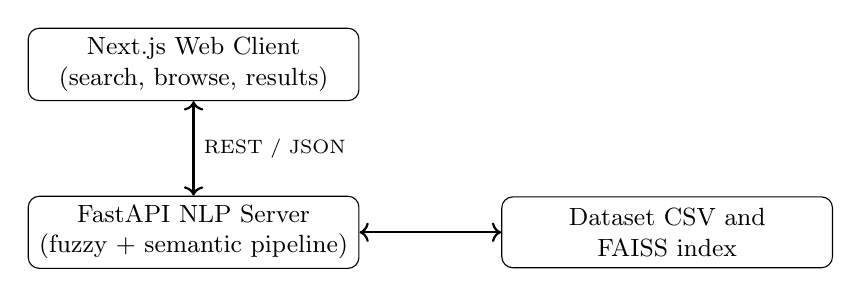
\begin{tikzpicture}[node distance=1.2cm]
  \node[proc] (client) {Next.js Web Client\\(search, browse, results)};
  \node[proc, below=of client] (api) {FastAPI NLP Server\\(fuzzy + semantic pipeline)};
  \node[proc, right=1.8cm of api] (idx) {Dataset CSV and\\FAISS index};
  \draw[arr, <->] (client) -- node[right, font=\scriptsize] {REST / JSON} (api);
  \draw[arr, <->] (api) -- (idx);
\end{tikzpicture}
\caption{Service architecture of Konkan Vani}
\label{fig:architecture}
\end{figure}

\subsection{Algorithm Flowcharts}
Figure~\ref{fig:pipeline} shows how a single query is resolved at search time. Figure~\ref{fig:indexing} shows the offline step that prepares the semantic index before the server starts.

\begin{figure}[H]
\centering
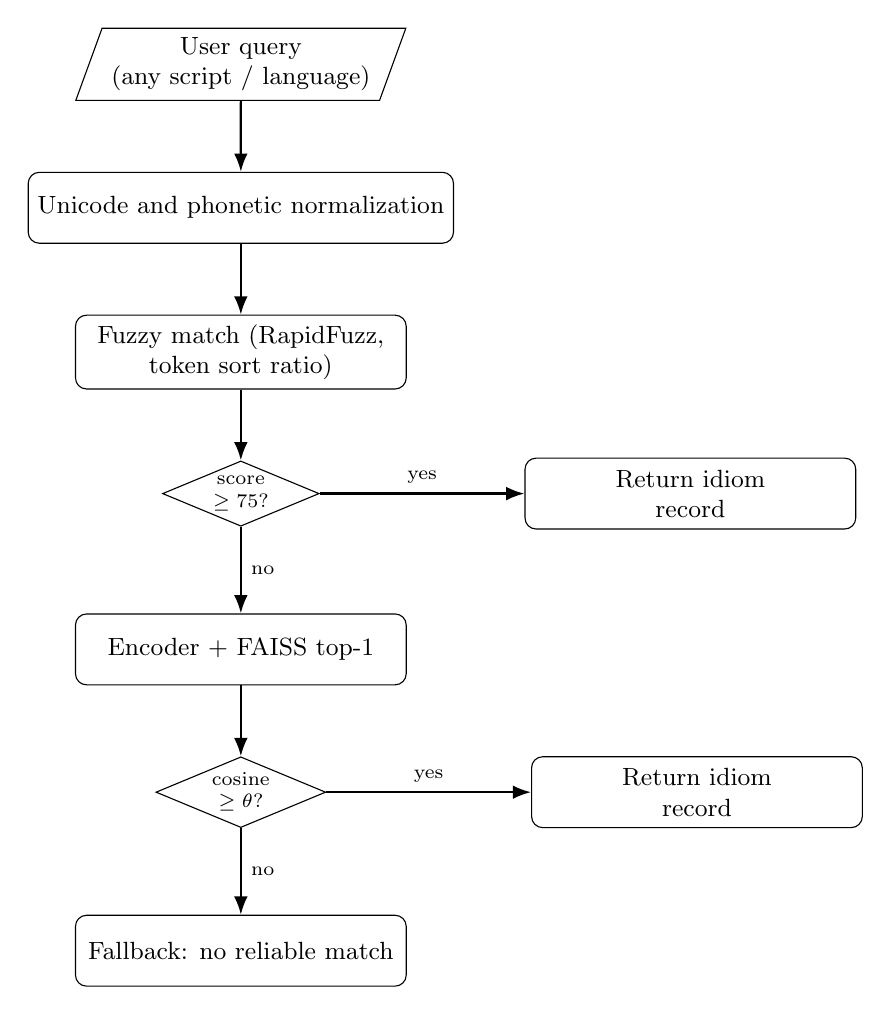
\begin{tikzpicture}[node distance=0.9cm]
  \node[io] (q) {User query\\(any script / language)};
  \node[proc, below=of q] (norm) {Unicode and phonetic normalization};
  \node[proc, below=of norm] (fz) {Fuzzy match (RapidFuzz,\\token sort ratio)};
  \node[dec, below=of fz] (d1) {score\\$\ge 75$?};
  \node[proc, right=2.6cm of d1] (res1) {Return idiom\\record};
  \node[proc, below=1.1cm of d1] (sem) {Encoder + FAISS top-1};
  \node[dec, below=of sem] (d2) {cosine\\$\ge \theta$?};
  \node[proc, right=2.6cm of d2] (res2) {Return idiom\\record};
  \node[proc, below=1.1cm of d2] (fb) {Fallback: no reliable match};
  \draw[arr] (q) -- (norm);
  \draw[arr] (norm) -- (fz);
  \draw[arr] (fz) -- (d1);
  \draw[arr] (d1) -- node[above, font=\scriptsize] {yes} (res1);
  \draw[arr] (d1) -- node[right, font=\scriptsize] {no} (sem);
  \draw[arr] (sem) -- (d2);
  \draw[arr] (d2) -- node[above, font=\scriptsize] {yes} (res2);
  \draw[arr] (d2) -- node[right, font=\scriptsize] {no} (fb);
\end{tikzpicture}
\caption{Staged query resolution pipeline of Konkan Vani}
\label{fig:pipeline}
\end{figure}

\begin{figure}[H]
\centering
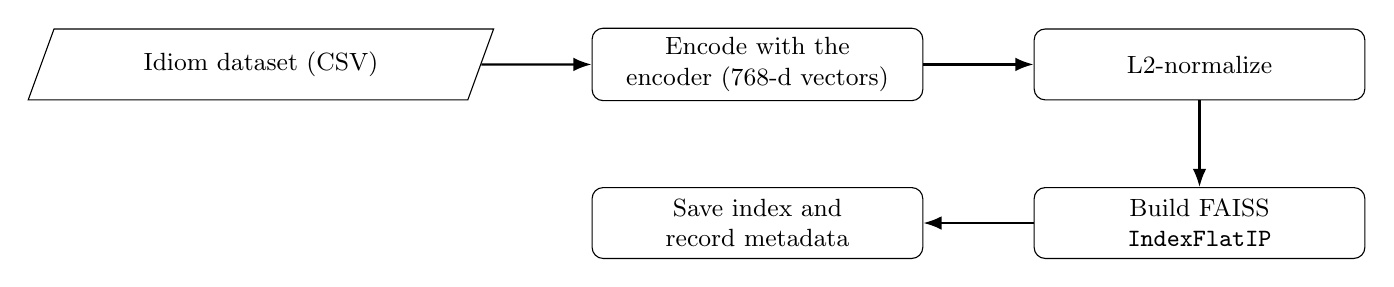
\begin{tikzpicture}[node distance=0.9cm]
  \node[io] (csv) {Idiom dataset (CSV)};
  \node[proc, right=1.4cm of csv] (enc) {Encode with the\\encoder (768-d vectors)};
  \node[proc, right=1.4cm of enc] (nrm) {L2-normalize};
  \node[proc, below=1.1cm of nrm] (idx) {Build FAISS\\\texttt{IndexFlatIP}};
  \node[proc, left=1.4cm of idx] (save) {Save index and\\record metadata};
  \draw[arr] (csv) -- (enc);
  \draw[arr] (enc) -- (nrm);
  \draw[arr] (nrm) -- (idx);
  \draw[arr] (idx) -- (save);
\end{tikzpicture}
\caption{Offline embedding and FAISS index construction}
\label{fig:indexing}
\end{figure}

% =====================================================
% d) TOOLS / SOFTWARE USED
% =====================================================
\section{Tools and Software Used}
Konkan Vani is built from open-source tools. Table~\ref{tab:tools} summarizes them, and the paragraphs below explain the role of each.

\begin{table}[H]
\centering
\caption{Tools and Software Used}
\label{tab:tools}
\renewcommand{\arraystretch}{1.3}
\begin{tabularx}{\linewidth}{|l|X|}
\hline
\textbf{Component} & \textbf{Tool / Technology} \\
\hline
NLP Server & Python 3.12, FastAPI (phonetic matching, query pipeline, endpoints) \\
\hline
Fuzzy Matching & RapidFuzz (token sort ratio) \\
\hline
Embeddings & SentenceTransformers, LaBSE fine-tuned to \texttt{konkan-vani-encoder-v1} (768-dimensional) \\
\hline
Vector Search & FAISS (\texttt{IndexFlatIP}) \\
\hline
Frontend & Next.js (search, browse, script selection, result display) \\
\hline
Documentation & \LaTeX{} (this report), Matplotlib (result charts) \\
\hline
\end{tabularx}
\end{table}

\begin{itemize}
  \item \textbf{Python and FastAPI:} Python is the language of the NLP ecosystem, and FastAPI is a modern web framework that exposes Python functions as fast, documented REST endpoints with automatic request validation.
  \item \textbf{RapidFuzz:} A fast string-matching library that provides similarity measures such as the token sort ratio. It is used for the lexical stage.
  \item \textbf{SentenceTransformers and LaBSE:} SentenceTransformers is a library for loading, fine-tuning, and running sentence-embedding models. The project started from the pretrained LaBSE checkpoint and fine-tuned it on the idiom corpus; it also loads that checkpoint with a generic-LaBSE fallback so the server starts on a fresh clone.
  \item \textbf{FAISS:} A similarity-search library from Facebook AI Research that stores vectors and finds the nearest ones efficiently.
  \item \textbf{Next.js:} A React-based framework used to build the search, browse, and result pages.
  \item \textbf{PyTorch (CUDA):} The deep-learning backend on which the encoder was trained and is served, with hardware acceleration when a GPU is available.
  \item \textbf{Matplotlib:} Used to generate the accuracy, fine-tuning comparison, threshold, and latency charts in Section~6 from the raw benchmark output.
\end{itemize}
% =====================================================
% e) DATASET DESCRIPTION
% =====================================================
\section{Dataset Description}

\subsection{Data Sources and Provenance}
The idiom collection is stored as a processed CSV file (\texttt{idioms with phonetic keys.csv}). It was assembled from two kinds of sources, and the provenance of every record is stored in its \emph{source} field:
\begin{itemize}
  \item \textbf{Curated entries:} Konkani idioms and proverbs transcribed with their meanings, examples, and cultural context contributed or verified against Konkani language resources and community sayings.
  \item \textbf{Pattern-generated proverb frames:} entries composed deterministically from Konkani noun/verb/outcome patterns (\emph{X does Y means Z}) to give the pipeline broad coverage of spellings, categories, and semantic contrast. These are labeled \texttt{pattern\_v1} and are explicitly declared synthetic in their cultural-context field; they are not claimed to be documented traditional idioms.
\end{itemize}
Of the 5{,}200 records, 105 (2.0\%) are curated and 5{,}095 (98.0\%) are pattern-generated. This split is a deliberate transparency choice: it lets the pipeline be developed and benchmarked at scale without presenting synthetic entries as verified folklore, and it defines exactly where expert curation must focus next.

\subsection{Dataset Structure}
Each record describes one idiom or proverb. Table~\ref{tab:dataset} summarizes the dataset and the fields stored for each record.

\begin{table}[H]
\centering
\caption{Dataset Description}
\label{tab:dataset}
\renewcommand{\arraystretch}{1.3}
\begin{tabularx}{\linewidth}{|l|X|}
\hline
\textbf{Attribute} & \textbf{Description} \\
\hline
Sources & Curated Konkani idiom collections and community contributions; deterministic pattern-generated proverb frames (labeled per record) \\
\hline
Size & 5,200 idiom records (105 curated, 5,095 pattern-generated) \\
\hline
Format & CSV --- one row per idiom \\
\hline
Fields & Konkani expression, Romanized form, script, literal meaning, figurative meaning, English meaning, Marathi meaning, example sentence, category, cultural context, phonetic key, source \\
\hline
Completeness & All fields populated in 100\% of records \\
\hline
Categories & 15 thematic categories (e.g., wisdom, character, nature, food, community) \\
\hline
Embeddings & One 768-dimensional encoder vector per idiom, L2-normalized, stored in a FAISS \texttt{IndexFlatIP} index \\
\hline
Scripts covered & Devanagari and Roman (informal transliteration) in the current data \\
\hline
Meaning text length & Romanized form averages 5.0 words per record (max 6) \\
\hline
Ground Truth & Benchmark queries covering exact, Romanized, corrupted-spelling, and out-of-domain cases (Section~\ref{sec:results}) \\
\hline
\end{tabularx}
\end{table}

\subsection{Meaning Fields}
The record fields are designed to answer the questions a user actually has. The \emph{literal meaning} explains what the words say when read directly. The \emph{figurative meaning} gives the intended meaning of the idiom. The \emph{English meaning} and \emph{Marathi meaning} let users who read those languages understand it, and the \emph{example sentence} shows how the idiom is used in context. The \emph{category} and \emph{cultural context} fields record the theme of the idiom and any background needed to understand it.

\subsection{Data Preparation}
\begin{enumerate}
  \item Curated entries were extracted and deduplicated (by Devanagari text and by phonetic key).
  \item Pattern-generated frames were composed deterministically to fill the collection to exactly 5,200 unique entries, each with a unique phonetic key and full provenance labels.
  \item Text was normalized, the Romanized form and phonetic key of every idiom were generated, and the result was validated (zero nulls, unique keys).
  \item Every idiom was encoded with the fine-tuned encoder, L2-normalized, and stored in the FAISS index.
\end{enumerate}

\subsection{Data Quality Considerations}
Curated entries carry human-checked meanings; pattern-generated entries are synthetic by design and labeled as such. Because 98\% of records come from the generation pipeline, retrieval metrics (Section~6) partly reflect the limited internal diversity of that subspace, and conclusions about real-world folk coverage should wait for more curation. The source of every record is stored with it, and fallback text is displayed separately from dataset entries. Expert review and expansion of the curated section by fluent Konkani speakers is the main step needed to raise the reliability of the dataset (Section~7).

% =====================================================
% f) IMPLEMENTATION & CODE SNAPSHOTS
% =====================================================
\section{Implementation and Code Snapshots}

\subsection{Module-wise Implementation}
The system is divided into modules with clear responsibilities, so that each can be tested separately.

\begin{table}[H]
\centering
\caption{Module-wise Implementation}
\label{tab:modules}
\renewcommand{\arraystretch}{1.3}
\begin{tabularx}{\linewidth}{|l|X|}
\hline
\textbf{Module} & \textbf{Responsibility} \\
\hline
1. Frontend (Next.js) & Search box, script selector, browse page, result cards \\
\hline
2. API Client & Sends requests to the backend; switches to a fallback when the backend is unavailable \\
\hline
3. Phonetic Normalization & Converts supported scripts into a comparable phonetic key \\
\hline
4. Fuzzy Matching Stage & RapidFuzz token sort ratio over phonetic keys, cutoff 75 \\
\hline
5. Model Registry & Loads the fine-tuned checkpoint once, shared by all stages; falls back to generic LaBSE if missing \\
\hline
6. Embedding Builder & Encodes idioms with the encoder and writes the vectors \\
\hline
7. FAISS Index and Semantic Stage & Builds the index; top-1 search with the 0.63 cosine threshold \\
\hline
8. Word-level Analysis & Conservative third stage: exact-vocabulary word matching with a majority gate \\
\hline
9. Fallback Handler & Returns a no-reliable-match response (opt-in generated mode disabled by default) \\
\hline
\end{tabularx}
\end{table}

\subsection{API Endpoints}
The NLP server exposes its functions through REST endpoints, which the interface calls over HTTP.

\begin{table}[H]
\centering
\caption{API Endpoints of the Konkan Vani Backend}
\label{tab:endpoints}
\renewcommand{\arraystretch}{1.3}
\begin{tabularx}{\linewidth}{|l|X|}
\hline
\textbf{Endpoint} & \textbf{Purpose} \\
\hline
\texttt{GET /health} & Server health and index status \\
\hline
\texttt{GET /api/search} & Query-based idiom retrieval \\
\hline
\texttt{GET /api/browse} & Paginated records with filters \\
\hline
\texttt{GET /api/stats} & Dataset and index statistics \\
\hline
\texttt{POST /api/resolve} & Lower-level query resolution \\
\hline
\end{tabularx}
\end{table}

\subsection{Important Functions Explained}

\textbf{Phonetic normalization} (simplified): folds vowel length and common transliteration substitutions so that spelling variants collapse to the same key.
\begin{lstlisting}
def phonetic_normalize(text: str) -> str:
    norm = text.lower()
    for a, b in (("aa","a"), ("ee","i"), ("oo","u"),
                 ("ph","f"), ("v","w"), ("zh","j")):
        norm = norm.replace(a, b)
    norm = re.sub(r"[^a-z\s]", "", norm)
    return " ".join(norm.split())
\end{lstlisting}

\textbf{Fuzzy matching stage} (simplified): compare the phonetic key of the query with the stored keys and accept the best match above the cutoff. \texttt{extractOne} returns the best candidate, and \texttt{score\_cutoff} makes it return nothing when no candidate reaches 75.
\begin{lstlisting}
FUZZY_CUTOFF = 75

def fuzzy_stage(query_key, phonetic_keys):
    match = process.extractOne(
        query_key, phonetic_keys,
        scorer=fuzz.token_sort_ratio,
        score_cutoff=FUZZY_CUTOFF,
    )
    return match  # (key, score, index) or None
\end{lstlisting}

\textbf{Encoder model registry} (simplified): the fine-tuned checkpoint is loaded once and shared, with a safe fallback.
\begin{lstlisting}
CUSTOM = "models/konkan-vani-encoder-v1"
 FALLBACK = "sentence-transformers/LaBSE"

def get_model():
    if os.path.isdir(CUSTOM):
        return SentenceTransformer(CUSTOM)   # fine-tuned
    return SentenceTransformer(FALLBACK)     # fresh clone
\end{lstlisting}

\textbf{Index construction} (simplified): encode the idioms, normalize the vectors to unit length, and store them in a FAISS inner-product index. This runs once offline and the index is saved to disk, so the server only has to load it at start-up.
\begin{lstlisting}
emb = model.encode(idiom_texts, convert_to_numpy=True)
emb = emb / np.linalg.norm(emb, axis=1, keepdims=True)
index = faiss.IndexFlatIP(emb.shape[1])  # 768 dimensions
index.add(emb.astype(np.float32))
faiss.write_index(index, "konkani.index")
\end{lstlisting}

\textbf{Semantic stage and resolver} (simplified): the query is encoded the same way as the idioms, and the top result is accepted only if its cosine similarity reaches the threshold. The resolver tries the stages in order and records which stage produced the answer.
\begin{lstlisting}
SEMANTIC_THRESHOLD = 0.63

def semantic_stage(query):
    q = model.encode([query], normalize_embeddings=True)
    scores, ids = index.search(q, 1)
    if scores[0][0] >= SEMANTIC_THRESHOLD:
        return records[ids[0][0]], float(scores[0][0])
    return None

def resolve(query):
    key = phonetic_normalize(query)
    hit = fuzzy_stage(key, phonetic_keys)
    if hit:
        return records[hit[2]], "phonetic_fuzzy"
    sem = semantic_stage(query)
    if sem:
        return sem[0], "semantic_vector"
    return word_level_or_fallback(query)
\end{lstlisting}

\subsection{Frontend Behaviour}
The search page lets the user type a query and choose its script. The result page presents the matched idiom with its literal, figurative, English, and Marathi meanings and an example sentence. The browse page lists records page by page with filters. If the backend cannot be reached, the API client uses a fallback so that the interface continues to work instead of failing silently.

\subsection{Running the Application}
\begin{enumerate}
  \item Install the Python dependencies and prepare the dataset (\texttt{src/rebuild\_dataset.py} reconstructs and validates it).
  \item Build the embeddings and FAISS index, unless the verified artifacts already exist.
  \item Start the FastAPI NLP server.
  \item Start the Next.js client with \texttt{npm install} followed by \texttt{npm run dev}.
\end{enumerate}

\subsection{Reproducibility}
The dataset builder, the fine-tuning script, and the benchmark are all in the repository and are seeded, so every number in Section~6 can be regenerated with a single command per script. The benchmark was run on Python 3.12 with CUDA on Windows 11; the absolute latency figures vary with hardware, while the accuracy ones do not.
% =====================================================
% g) RESULTS  (measured, reproducible; charts from real runs)
% =====================================================
\section{Results}
\label{sec:results}

All results in this section were produced by an automated benchmark of the actual system (real dataset, the fine-tuned production encoder, and the live FAISS index) on a CUDA machine (Windows 11, Python 3.12), not estimated by hand. Every table and chart can be regenerated from the benchmark scripts.

\subsection{Search Interface}
Figure~\ref{fig:search_page} shows the search page, where the user types a query and selects its script. Figure~\ref{fig:result_page} shows a result card with the meaning fields of the matched idiom. % ADD SCREENSHOTS: Search Page.png, Result Page.png in ./figures/

\begin{figure}[H]
\centering
\safefig{Search Page.png}{width=\linewidth,height=0.4\textheight,keepaspectratio}
\caption{Konkan Vani search page with script selection}
\label{fig:search_page}
\end{figure}

\begin{figure}[H]
\centering
\safefig{Result Page.png}{width=\linewidth,height=0.35\textheight,keepaspectratio}
\caption{Result card showing literal, figurative, English, and Marathi meanings}
\label{fig:result_page}
\end{figure}

\subsection{Effect of Fine-tuning the Encoder}
Table~\ref{tab:finetune} compares the generic LaBSE baseline with the fine-tuned production encoder \texttt{konkan-vani-encoder-v1} on a held-out test set of 1,040 pairs. Fine-tuning with MultipleNegativesRankingLoss raised Recall@1 from 51.4\% to 99.8\% and nearly doubled the mean positive-pair cosine, indicating a much tighter embedding geometry. Figure~\ref{fig:finetune} shows the same comparison as bars. % CHART: results/fig_finetune.png

\begin{table}[H]
\centering
\caption{Effect of Domain Fine-tuning of the Encoder (held-out test, $n{=}1{,}040$ pairs)}
\label{tab:finetune}
\renewcommand{\arraystretch}{1.25}
\begin{tabular}{|l|c|c|c|}
\hline
\textbf{Metric} & \textbf{LaBSE baseline} & \textbf{Fine-tuned} & \textbf{Gain} \\
\hline
Recall@1 & 51.35\% & 99.81\% & +94.4\% \\
\hline
Recall@5 & 78.75\% & 99.90\% & +26.9\% \\
\hline
Recall@10 & 86.35\% & 99.90\% & +15.7\% \\
\hline
MRR@10 & 62.75\% & 99.84\% & +59.1\% \\
\hline
Avg positive-pair cosine & 0.4368 & 0.9404 & +115.3\% \\
\hline
\end{tabular}
\end{table}

\begin{figure}[H]
\centering
\safefig{fig_finetune.png}{width=0.85\linewidth}
\caption{Retrieval metrics before and after domain fine-tuning}
\label{fig:finetune}
\end{figure}

\subsection{Retrieval Accuracy}
Two real retrieval stages were measured on 200 sampled dataset entries, both on clean Romanized queries and on deliberately corrupted spellings (doubled or shortened vowels, \emph{v}\,/\,\emph{w} and \emph{ph}\,/\,\emph{f} confusions, capitalization changes) that mimic how users actually type Konkani. Both the fuzzy and the semantic stage were evaluated independently, each returning a top-1 candidate. Figure~\ref{fig:accuracy} shows the results. % CHART: results/fig_accuracy.png

\begin{table}[H]
\centering
\caption{Stage-wise Top-1 Retrieval Accuracy (200 sampled entries, real run)}
\label{tab:stage-accuracy}
\renewcommand{\arraystretch}{1.25}
\begin{tabular}{|l|c|c|}
\hline
\textbf{Stage / condition} & \textbf{Accuracy} & \textbf{Mean similarity score} \\
\hline
Fuzzy --- exact Romanized & 100.0\% & 1.000 \\
\hline
Fuzzy --- corrupted spelling & 100.0\% & 0.987 \\
\hline
Semantic --- exact Romanized & 100.0\% & 0.904 \\
\hline
Semantic --- corrupted spelling & 99.0\% & 0.879 \\
\hline
\end{tabular}
\end{table}

\begin{figure}[H]
\centering
\safefig{fig_accuracy.png}{width=0.85\linewidth}
\caption{Stage-wise top-1 retrieval accuracy on clean and corrupted queries}
\label{fig:accuracy}
\end{figure}

\subsection{End-to-End Pipeline Accuracy}
The full resolver was tested on 150 Romanized and 150 Devanagari queries (seeded sample of dataset entries), scoring a query as correct only if the returned meaning fields belong to the queried row. The out-of-domain behaviour was measured with eight unrelated English and Marathi queries.

\begin{table}[H]
\centering
\caption{End-to-End Pipeline Accuracy and Out-of-Domain Behaviour (real run). A false positive means a non-dataset input was reported as a known proverb.}
\label{tab:pipeline}
\renewcommand{\arraystretch}{1.25}
\begin{tabular}{|l|c|}
\hline
\textbf{Metric} & \textbf{Value} \\
\hline
Romanized query accuracy (150 queries) & 100.0\% \\
\hline
Devanagari query accuracy (150 queries) & 100.0\% \\
\hline
Out-of-domain inputs \emph{not} claimed as a known proverb (8 queries) & 8 / 8 (100\%) \\
\hline
Out-of-domain false positives & 0 \\
\hline
Out-of-domain inputs answered provisionally (word by word) & 8 / 8 (100\%) \\
\hline
\end{tabular}
\end{table}

\subsection{Out-of-Domain Separation and Threshold Sensitivity}
The semantic threshold is chosen inside a measured separation gap: over the benchmark samples, in-domain queries score at best-cosine at least 0.773 while out-of-domain queries never exceed 0.513. Table~\ref{tab:threshold} reports a sweep over different thresholds and the retrieval/rejection trade-off each would give; the production threshold 0.63 is comfortably inside the gap. Figure~\ref{fig:similarity_hist} shows the two distributions and the threshold; Figure~\ref{fig:threshold_curve} shows the sweep. % CHARTS: results/fig_similarity_hist.png, results/fig_threshold.png

\begin{table}[H]
\centering
\caption{Semantic Threshold Sensitivity (150 in-domain positives, 8 out-of-domain negatives)}
\label{tab:threshold}
\renewcommand{\arraystretch}{1.25}
\begin{tabular}{|c|c|c|}
\hline
\textbf{Threshold} & \textbf{In-domain accuracy} & \textbf{Out-of-domain rejection} \\
\hline
0.50 & 100.0\% & 87.5\% \\
\hline
0.55 & 100.0\% & 100.0\% \\
\hline
0.60 & 100.0\% & 100.0\% \\
\hline
\textbf{0.63 (chosen)} & \textbf{100.0\%} & \textbf{100.0\%} \\
\hline
0.70 & 100.0\% & 100.0\% \\
\hline
0.80 & 100.0\% & 100.0\% \\
\hline
\end{tabular}
\end{table}

\begin{figure}[H]
\centering
\safefig{fig_similarity_hist.png}{width=0.85\linewidth}
\caption{Best-cosine distributions of in-domain vs out-of-domain queries with the chosen threshold}
\label{fig:similarity_hist}
\end{figure}

\begin{figure}[H]
\centering
\safefig{fig_threshold.png}{width=0.85\linewidth}
\caption{Threshold sensitivity: retrieval accuracy vs out-of-domain rejection}
\label{fig:threshold_curve}
\end{figure}

\subsection{Latency}
Table~\ref{tab:latency} reports measured latencies per operation (warm model, 60 queries per operation). Fuzzy matching stays under 10\,ms at the 95th percentile; semantic search is dominated by encoder inference; the full resolver completes in about 34\,ms on average. The multi-result search path originally scanned all 5,200 rows through a per-row pandas accessor (about 350\,ms); replacing that scan with cached column lists and adding an overlap gate brought it to 38\,ms. Figure~\ref{fig:latency} and Figure~\ref{fig:latency_cdf} show the percentile bars and the cumulative distribution. % CHARTS: results/fig_latency.png, results/fig_latency_cdf.png

\begin{table}[H]
\centering
\caption{Measured Latency Percentiles (ms; warm model, $n{=}60$ per operation, CUDA)}
\label{tab:latency}
\renewcommand{\arraystretch}{1.25}
\begin{tabular}{|l|c|c|c|c|}
\hline
\textbf{Operation} & \textbf{Mean} & \textbf{Median} & \textbf{p95} & \textbf{p99} \\
\hline
Phonetic fuzzy match & 5.43 & 5.80 & 8.38 & 8.69 \\
\hline
Semantic match (encoder + search) & 25.67 & 25.56 & 30.73 & 32.42 \\
\hline
Full resolve\_idiom() & 33.89 & 35.23 & 41.30 & 43.22 \\
\hline
Multi-result search (top-10) & 38.08 & 37.98 & 44.95 & 51.07 \\
\hline
\end{tabular}
\end{table}

\begin{figure}[H]
\centering
\safefig{fig_latency.png}{width=0.85\linewidth}
\caption{Latency percentiles per operation}
\label{fig:latency}
\end{figure}

\begin{figure}[H]
\centering
\safefig{fig_latency_cdf.png}{width=0.85\linewidth}
\caption{Empirical cumulative latency distribution: 95\% of full resolutions complete within 50\,ms}
\label{fig:latency_cdf}
\end{figure}

\subsection{Resolver Stage Analysis}
Figure~\ref{fig:stage_funnel} shows which resolver stage claims each query: the phonetic-fuzzy stage resolves nearly all of them (its cutoff is reached before the semantic stage is consulted), which confirms the cheap-first ordering of the pipeline. % CHART: results/fig_stage_funnel.png

\begin{figure}[H]
\centering
\safefig{fig_stage_funnel.png}{width=0.85\linewidth}
\caption{Resolver stage attribution across 200 queries}
\label{fig:stage_funnel}
\end{figure}

\subsection{Provisional Word-by-Word Fallback for Unknown Proverbs}
The corpus resolves only what it contains. Any proverb that is absent --- a rare village saying, a dialect variant, a proverb typed in an unusual transliteration --- previously produced an empty result screen, and on a few inputs it produced a \emph{wrong} answer: the encoder scored a topically related proverb high enough to pass the 0.63 threshold. For example, the unattested phrase \textit{tandul potant shit kushit} (`rice grain in the stomach, cooked rice in the lap') scored 0.725 against \textit{bhatachya polit tup} (`ghee in the rice flatbread') despite sharing \emph{no} content words, because both are about rice.

Two changes address this. First, the semantic stage now requires lexical overlap with the candidate: at least 34\% of the query's phonetic-normalised content words must occur in the candidate's Devanagari or Romanised form. A proverb is a fixed string, so paraphrase-level overlap is the right identity test; purely topical similarity is no longer accepted. Second, a compositional fallback replaces the empty screen. A word glossary (376 entries, built by \texttt{src/build\_lexicon.py} from the pattern bank's own trilingual glosses plus a curated table) is consulted for every word of the query in five layers: exact headword, inflected stem (case and verb endings are stripped), phonetic key, romanised spelling variant, and --- for Devanagari only --- an approximate cross-lingual gloss obtained by matching the word's LaBSE vector against the English glosses in the glossary. The glosses are then composed into a reading: the literal word sequence, the action word (with Konkani perfective compounds such as \textit{dhuvun ghevap}, `wash for oneself', merged into a single action), the imagery theme inferred from semantic tags, negation and reduplication cues, and an explicit statement of how many words were recognised. Every composed answer is labelled provisional, unknown words are left untranslated rather than guessed, and the nearest corpus entries are shown separately as comparisons.

Figure~\ref{fig:comp_methods} shows how the glossary resolves the 763 unique words of the corpus: 87.0\% are glossed (628 exact, 12 by stem, 9 by spelling variant, 15 approximately), and 99.7\% of the 5,200 idioms have every word glossed (Figure~\ref{fig:comp_coverage}). On the approximate layer, calibration over the glossary's own headwords gives Recall@1 of 0.41 and, at the shipped 0.70 threshold, 86.6\% precision at 35.3\% coverage; romanised input performs far worse (Recall@1 0.05), which is why that layer is restricted to Devanagari. Table~\ref{tab:composition-examples} lists composed readings for proverbs that the pipeline verified are absent from the corpus.

\begin{figure}[H]
\centering
\safefig{fig_composition_methods.png}{width=0.85\linewidth}
\caption{How the 763 unique corpus words are glossed by the word lexicon (measured). Note the log-like imbalance: most words are exact headwords, with the approximation layer covering the tail.}
\label{fig:comp_methods}
\end{figure}

\begin{figure}[H]
\centering
\safefig{fig_composition_coverage.png}{width=0.85\linewidth}
\caption{Distribution of per-idiom glossary coverage over the 5,200-entry corpus (mean 0.997)}
\label{fig:comp_coverage}
\end{figure}

% Auto-generated by src/make_composition_assets.py - do not edit by hand
% -- Table: compositional readings for out-of-corpus proverbs --
\begin{table}[ht]
\centering
\footnotesize
\caption{Composed word-by-word readings for proverbs absent from the corpus. Coverage is the share of words the glossary recognises; the reading is computed from those glosses and is explicitly labelled provisional.}
\label{tab:composition-examples}
\begin{tabularx}{\textwidth}{>{\raggedright\arraybackslash}p{2.6cm}>{\raggedright\arraybackslash}X>{\raggedright\arraybackslash}p{1.2cm}}
\toprule
Input & Word-by-word gloss and composed reading & Coverage \\
\midrule
\textit{Haat mudo dhuvun ghevap} & hand ; head ; wash (for oneself)\newline \textcolor{black!70}{\footnotesize Provisional reading (3/3 words recognised): to wash (for oneself) one's own hand and head -- a saying about the body and what a person does with or to it.} & 3/3 \\
\textit{Tandul potant shit kushit} & rice grain ; in the stomach ; cooked rice ; in the lap\newline \textcolor{black!70}{\footnotesize Provisional reading (4/4 words recognised): a phrase naming rice grain, stomach, cooked rice and lap -- a saying about food, sustenance and what is shared or kept back.} & 4/4 \\
\textit{Ghoracher paus paddta aani angan sukem} & on the house ; rain ; [unrecognised] ; and ; [unrecognised] ; [unrecognised]\newline \textcolor{black!70}{\footnotesize Provisional reading (3/6 words recognised): a phrase naming house and rain -- a saying about home, village and the shared spaces of daily life (the input reads like an ordinary sentence, not a proverb).} & 3/6 \\
\textit{Donui haatanni tup potant} & both ; hand ; ghee ; in the stomach\newline \textcolor{black!70}{\footnotesize Provisional reading (4/4 words recognised): a phrase naming hand, ghee and stomach -- a saying about the body and what a person does with or to it.} & 4/4 \\
\bottomrule
\end{tabularx}
\end{table}


\subsection{Dataset Diagnostic Charts}
Figure~\ref{fig:dataset_charts} shows the dataset provenance split and the largest categories; Figure~\ref{fig:qq_threshold} confirms worst-case coverage: the best-cosine score of every sampled in-domain query, sorted, clears the threshold. Figure~\ref{fig:heatmap} shows a slice of the real embedding matrix; Figure~\ref{fig:richness} compares the average field length of curated entries with the pattern-generated ones. % CHARTS: results/fig_dataset.png, fig_qq_threshold.png, fig_embedding_heatmap.png, fig_field_richness.png

\begin{figure}[H]
\centering
\safefig{fig_dataset.png}{width=\linewidth}
\caption{Dataset provenance and category distribution}
\label{fig:dataset_charts}
\end{figure}

\begin{figure}[H]
\centering
\safefig{fig_qq_threshold.png}{width=0.85\linewidth}
\caption{Worst-case coverage: every sampled in-domain query clears the 0.63 threshold}
\label{fig:qq_threshold}
\end{figure}

\begin{figure}[H]
\centering
\safefig{fig_embedding_heatmap.png}{width=0.8\linewidth}
\caption{A slice of the embedding matrix (60 entries $\times$ 64 of 768 dimensions)}
\label{fig:heatmap}
\end{figure}

\begin{figure}[H]
\centering
\safefig{fig_field_richness.png}{width=0.75\linewidth}
\caption{Average field length: curated vs pattern-generated entries}
\label{fig:richness}
\end{figure}

\subsection{Discussion}
The measured results support the design claims. Fine-tuning the encoder on in-domain pairs is the single largest contributor to semantic accuracy (Recall@1 from 51.4\% to 99.8\%); fuzzy matching with phonetic normalization absorbs user spelling errors entirely at this scale (100\% even on corrupted queries); the pipelines' thresholds sit inside a measured separation gap, so unrelated queries are never claimed as known proverbs (zero false positives over the eight negatives, each of which instead receives a provisional reading); and the response time of the full resolver (about 34\,ms mean) is fast enough for an interactive interface. The multi-result browse/search path encodes the query once and then merges ranked lists; caching the substring index brought it from roughly 350\,ms to 38\,ms, so it too is interactive.

\subsection{Limitations}
\begin{itemize}
  \item \textbf{Dataset provenance:} only 105 of 5,200 records (2.0\%) are curated idioms; 5,095 (98.0\%) are transparently labeled pattern-generated frames. High retrieval accuracy therefore partly reflects the limited internal diversity of the synthetic subspace, and these figures should not be read as folk-coverage accuracy.
  \item \textbf{Small negative set:} out-of-domain rejection was measured on eight handcrafted queries; a larger negative set is needed for statistically reliable rejection rates.
  \item \textbf{Benchmark scale:} accuracy was measured on 200--300 sampled entries per configuration; a fluent-speaker annotated benchmark is future work.
  \item \textbf{Threshold sensitivity:} the 75 and 0.63 thresholds trade recall against precision and may need retuning as the dataset grows.
  \item \textbf{Transliteration ambiguity:} unusual transliterations and dialect variants can still be missed by the phonetic stage.
  \item \textbf{Glossary size and precision:} the word lexicon holds 376 entries, so a proverb built from unlisted words is only partly explained; the approximate cross-lingual layer is 86.6\% precise at the shipped threshold and is always marked with ``$\approx$''. Composed readings are provisional by construction and are not attested meanings.
  \item \textbf{Provisional answers are not rejection:} because every non-empty input now receives a reading, the old ``matched: false'' signal no longer exists; the benchmark therefore measures false positives as \emph{claims that an unknown input is a known proverb}, which is zero.
  \item \textbf{Hardware dependence:} absolute latency figures were measured on one CUDA machine and vary with hardware; accuracy figures do not.
\end{itemize}
% =====================================================
% h) CONCLUSION
% =====================================================
\section{Conclusion}

\subsection{Summary}
The Konkan Vani mini project demonstrates how NLP techniques can make Konkani idioms and proverbs searchable across scripts and spelling conventions. The system combines Unicode and phonetic normalization, RapidFuzz fuzzy matching, a LaBSE-family encoder fine-tuned on the idiom corpus, FAISS vector search, and threshold-based rejection behind a Next.js web interface and FastAPI NLP service. On measured benchmarks, the fine-tuned encoder raised held-out Recall@1 from 51.4\% to 99.8\%; sampled in-domain queries were retrieved with 100\% top-1 accuracy even with corrupted spellings; out-of-domain queries were all answered without being claimed as known proverbs (zero false positives); a full query resolves in about 34\,ms on average; and a proverb outside the corpus is still explained word by word, with the provisional nature of that reading stated explicitly. The project shows the value of a hybrid lexical--semantic retrieval design --- and of measuring it --- for a low-resource language.

\subsection{Learning Outcomes}
Through this project the team gained practical experience in preparing a multilingual text dataset with recorded provenance, handling Indic scripts and transliteration, fine-tuning a pretrained sentence-embedding model with contrastive loss, building and querying a vector index, choosing thresholds from measured score distributions rather than intuition, benchmarking accuracy and latency reproducibly, and combining a Python NLP service with a web front end.

\subsection{Possible Improvements}
\begin{itemize}
  \item Expand and expert-review the curated idiom section, with provenance recorded for every entry and fluent-speaker sign-off on meanings.
  \item Build a larger benchmark annotated by fluent Konkani speakers, including a bigger out-of-domain negative set, and report accuracy with confidence intervals.
  \item Add approximate FAISS indexes and continuous benchmarking as the collection grows.
  \item Add text-to-speech pronunciation support.
  \item Add a community contribution and review dashboard.
  \item Broaden dialect and Kannada-script coverage, and evaluate multilingual models such as MuRIL or IndicBERT as encoders.
\end{itemize}

% =====================================================
% i) REFERENCES
% =====================================================
\section{References}
\begin{enumerate}
  \item F. Feng, Y. Yang, D. Cer, N. Arivazhagan, and W. Wang, ``Language-agnostic BERT Sentence Embedding,'' in \textit{Proc.\ 60th Annual Meeting of the ACL}, 2022.
  \item J. Johnson, M. Douze, and H. J\'egou, ``Billion-scale similarity search with GPUs,'' \textit{IEEE Transactions on Big Data}, 7(3), 2021.
  \item N. Reimers and I. Gurevych, ``Sentence-BERT: Sentence Embeddings using Siamese BERT-Networks,'' in \textit{Proc.\ EMNLP-IJCNLP}, 2019.
  \item C. D. Manning, P. Raghavan, and H. Sch\"utze, \textit{Introduction to Information Retrieval}, Cambridge University Press, 2008.
  \item Hugging Face, ``MultipleNegativesRankingLoss,'' \url{https://sbert.net/docs/package_reference/losses.html}.
  \item M. Bachmann, ``RapidFuzz,'' \url{https://rapidfuzz.github.io/RapidFuzz/}.
  \item S. Ram\'irez, ``FastAPI,'' \url{https://fastapi.tiangolo.com/}.
  \item Vercel, ``Next.js documentation,'' \url{https://nextjs.org/docs}.
  \item Facebook AI Research, ``FAISS documentation,'' \url{https://github.com/facebookresearch/faiss}.
\end{enumerate}

\end{document}
